\documentclass{sig-alternate}
%\documentclass[11pt,letterpaper,singlecolumn]{article}
%\usepackage{url}
\usepackage{epsfig}
%\usepackage{subfigure}
%%\usepackage{latexsym}
%%\usepackage{times}
%%\usepackage{fancyhdr}
%%\usepackage{multirow}
%\usepackage{listing}
\usepackage{soul}
\usepackage{algorithmic}
\usepackage{algorithm}
\usepackage{hyperref}

\newcommand{\parbold}[1]{\noindent{\bf #1}}
%%%%%%%%%%%%%%%%%%%%%%%%%%
%%% Remarks
\newif\ifremark
\long\def\remark#1{
\ifremark%
        \begingroup%
        \dimen0=\columnwidth
        \advance\dimen0 by -1in%
        \setbox0=\hbox{\parbox[b]{\dimen0}{\protect\em #1}}
        \dimen1=\ht0\advance\dimen1 by 2pt%
        \dimen2=\dp0\advance\dimen2 by 2pt%
        \vskip 0.25pt%
        \hbox to \columnwidth{%
                \vrule height\dimen1 width 3pt depth\dimen2%
                \hss\copy0\hss%
                \vrule height\dimen1 width 3pt depth\dimen2%
        }%
        \endgroup%
\fi}

%%%%%%%%%%%%%%%%%%%%%%%%%%
%%% Block comments
\newcommand{\ignore}[1]{}

%%%%%%%%%%%%%%%%%%%%%%%%%%%%%%%%%%%%%
\remarkfalse
%\remarkfalse
% \remark{this is a comment that shows up in text
% Switch remarkfalse on to turn comments off } 
% -- use in body, not up here
%%%%%%%%%%%%%%%%%%%%%%%%%%%%%%%%%%%%%


\begin{document}


\title{ Honeypot Configuration and Data Analysis }
\author{Jared Campbell\\The University of Texas at Austin  \and David Zehden\\The University of Texas at Austin}

\pagenumbering{arabic}
%\date{}  % comment this out if you want the date to print

\maketitle

\begin{abstract}
This project aims to build a honeypot server and analyze the data it collects. The goal of a honeypot server is to create vulnerable server on the open internet which we expect will be attacked by malicious actors. These attacks will be logged by the server, then we will analyze the data collected to find common trends in the attacks. Our honeypot will collect data on both an attacking machine and the attacks it directs at the honeypot. Our honeypot server is hosted on an Amazon Web Services (AWS) virtual server instance. The network for the server has been configured to allow all incoming traffic on monitored ports we expect to be targeted (such as SSH). We then analyzed the collected data using Python to find trends in attacker IP addresses, attacker operating systems, attacked ports, and timing of attacks. The honey pot was successful in collecting a large amount of attack data, averaging over 1000 unique data points per day. Our research has determined that a honeypot server is an effective tool for monitoring potential attacks on a network. We have also found honeypots to be highly configurable which allows for the collection of data specific to an organization's needs. 
 
\end{abstract}

\section{Introduction}
\label{sec:intro}
A honeypot is a server that is made intentionally vulnerable in order to attract the attention of malicious actors. The server then logs any attempts by attackers to exploit and gain access to it. The goal is for researchers to be able to analyze common trends in the kinds of attacks used by malicious actors and even possibly discover new kinds of attacks that have never been seen before. Another use case for honeypots in an enterprise environment is to slow down attackers by allowing them to attack the non-critical honeypot instead critical infrastructure. 

There are many different tools that can be used to create a honeypot. For example, the honeypot could emulate a vulnerable web app or a vulnerable end-user machine. The configuration of the honeypot depends on the goals of its creators, whether that be research or protection as described above. Our goal is to research these various tools and configurations, and to gather enough data to be able provide an analysis of current trends in attacks. Since there are so many different tools and honeypot configurations, our implementation will focus on a general honeypot meant to collect as much data as possible. The results of our research will demonstrate the effectiveness of a honeypot in collecting different types of data which could be used to improve the security of an organization and provide knowledge on general trends to the information security community. 

For our approach, we have configured a honeypot as a vulnerable server using various tools which we have found to emulate common vulnerabilities and log attack data. We have also configured a front end website for the honeypot. The collected data is automatically analyzed and visualized via Python scripts, and the results are displayed on the website. The most interesting part of our design is that once the honeypot is configured, it runs continually without any need for further user interaction. The longer the honeypot runs, the more data it collects, and the more accurate trends over time become. As we were only able to run our fully configured honeypot for approximately one week, the analysis only shows common trends over a one week time period. However, given more time, the honeypot could eventually demonstrate trends over months or even years. The longer the honeypot is active, the more interesting the data becomes. 

In our initial results, we were able to track the top attacker IP addresses and their country of origin, attacker operating systems, targeted ports, timing of attacks, and SSH attack data such as the top usernames and passwords of all login attempts. Interestingly, the top five countries from which attacks originated were the United States, Netherlands, Russia, China, and Romania (in order of number of detections). The two most widely used operating systems by attackers were Linux 2.2.x-3.x and Windows 7 or 8 (respectively). It is interesting that attackers are using fairly outdated operating systems (current Linux kernel is 4.14 and Windows 7 will reach end of life in January 2020). 

In the future, we would like to continue to run the honeypot server in order to collect data over a larger time period. It will be interesting to see how trends change across weeks and months as well as overall long-term trends. There is also much more we could configure on the honeypot, such as making masking certain elements of the honeypot detection programs to make the honeypot seem like a more realistic target. We theorize that the more enticing the honeypot looks to attackers, the more likely they would be to attack it and possibly even use more advanced attacks, all of which would provide us with even more detailed data. 

\section{Motivation}
\label{sec:motivation}
%--------------------------------------------
\begin{figure}[t]
\begin{center}
\vspace{-0.2in}
%%\psfig{figure=1bcounter.eps,width=2.5in,height=1.8in} 
\psfig{figure=1bcounter.eps,width=1.7in,height=1.2in} 
\caption{A 1-bit counter with reset. With the conventional technique of OR-ing all input shadow values, the feedback loop ensures that a 
counter shall never be trusted once it gets marked as untrusted. Our shadow logic is more precise and recognizes that a trusted reset 
guarantees a trusted $0$ in the counter value.}
\label{fig:1bcounter}
\end{center}
\end{figure}
%--------------------------------------------

Motivation describes the most important of the related works. The ones that 
you either build on, prove/disprove, or in any way ``extend''. 

Other related work, that is orthogonal to your approach but is in the same
general problem-area, can be included in a separate related work section.
One good place for that is at the end, so it doesn't disrupt the story here.


% \ignore{comment text} is better than a line comment.
\ignore{Sometimes background is merged into motivation, and is not required separately.}

\section{Our Architecture}
\label{sec:arch}
We have set up a basic Amazon Web Services server. The server is an EC2 t2.micro instance. We are using an Ubuntu Server 18 image as our operating system. 

To create the functionality of the honeypot, we have found several tools which we will configure and test. \href{https://github.com/DinoTools/dionaea}{Dionaea} captures malware and can simulate certain individual vulnerabilities. \href{https://github.com/mushorg/snare}{SNARE} is a web application based honeypot which we plan on using for the face of our honeypot. 

For data analysis we will mainly use Python to graph trends. \href{https://github.com/mushorg/tanner/}{Tanner} is another tool we can test which analyzes data specifically from SNARE, mentioned above. 


\section{Setup and Configuration}
\label{sec:setup}
We have set up Dionaea on our AWS server and it is successfully collecting logs. Some further configuration may be required in order to ensure that we are logging at an appropriate level. We also plan to install and configure more modules for Dionaea including some for logging and some for adding more vulnerabilities. We have installed Snare and are attempting to configure it to meet our needs. We have also configured the AWS server's firewall and security groups. Currently we are allowing all inbound network traffic on all ports and denying all outbound traffic. SSH access is restricted to our own SSH keys. Password logins are denied and root login is also denied. So far we have logged numerous attempts from scanners to log on to our service, and Dionaea has already captured a few malware binaries. 


\section{Results}
\label{sec:results}
Due to some technical issues, we had to reset our EC2 instance, thus the findings presented are those collected following the reset. As of the writing of this paper, we have received over 1,300 attacks on our honeypots. Modern Honeypot Network provides some useful high level statistics about our honeypots some of which may be seen in tables 1 and 2. Another interesting observation is that the vast majority of our data came from Snort, as over 1,200 attacks originated on our Snort honeypot.

We also found that 1433 was attacked significantly than any other port. This is likely due to port 1433's use as the default port for many SQL servers [TODO ADD CITATION].


\begin{table}[H]
	\resizebox{\columnwidth}{!}{%
	\begin{tabular}{|c|c|c|}
		\hline
		IP Address (truncated) & Country     & Number of attacks \\ \hline
		45.136                 & Germany     & 21                \\ \hline
		80.82.7                & Netherlands & 18                \\ \hline
		83.97.2                & Romania     & 17                \\ \hline
		89.248                 & Netherlands & 17                \\ \hline
		81.22.4                & Russia      & 16                \\ \hline
	\end{tabular}%
	}
\caption{Top Five Individual Detected IP Addresses} \label{tab:ips}
\end{table}

\begin{table}[H]
	\resizebox{\columnwidth}{!}{%
	\begin{tabular}{|c|c|c|}
		\hline
		Attacked Port & Number of Attacks & Common Port Use                                                                               \\ \hline
		1433          & 195               & SQL Server                                                                                    \\ \hline
		22            & 70                & SSH                                                                                           \\ \hline
		5060          & 68                & Clear Text SIP, VoIP                                                                          \\ \hline
		445           & 18                & Server Message Block                                                                          \\ \hline
		8545          & 17                & \begin{tabular}[c]{@{}c@{}}Remote Procedure Call interface\\ of Ethereum clients\end{tabular} \\ \hline
	\end{tabular}%
	}
\caption{Top Five Attacked Ports} \label{tab:ports}
\end{table}

Using the \href{https://github.com/pieqq/PyGeoIpMap}{PyGeoIpMap} library, we were also able to plot the approximate locations of attacker IP addresses (Figure 1). From this plot, we can see that attacks came from all over the world, though were particularly prominent from East/South East Asia, Brazil, and various parts of Europe.

\begin{figure}[H]
	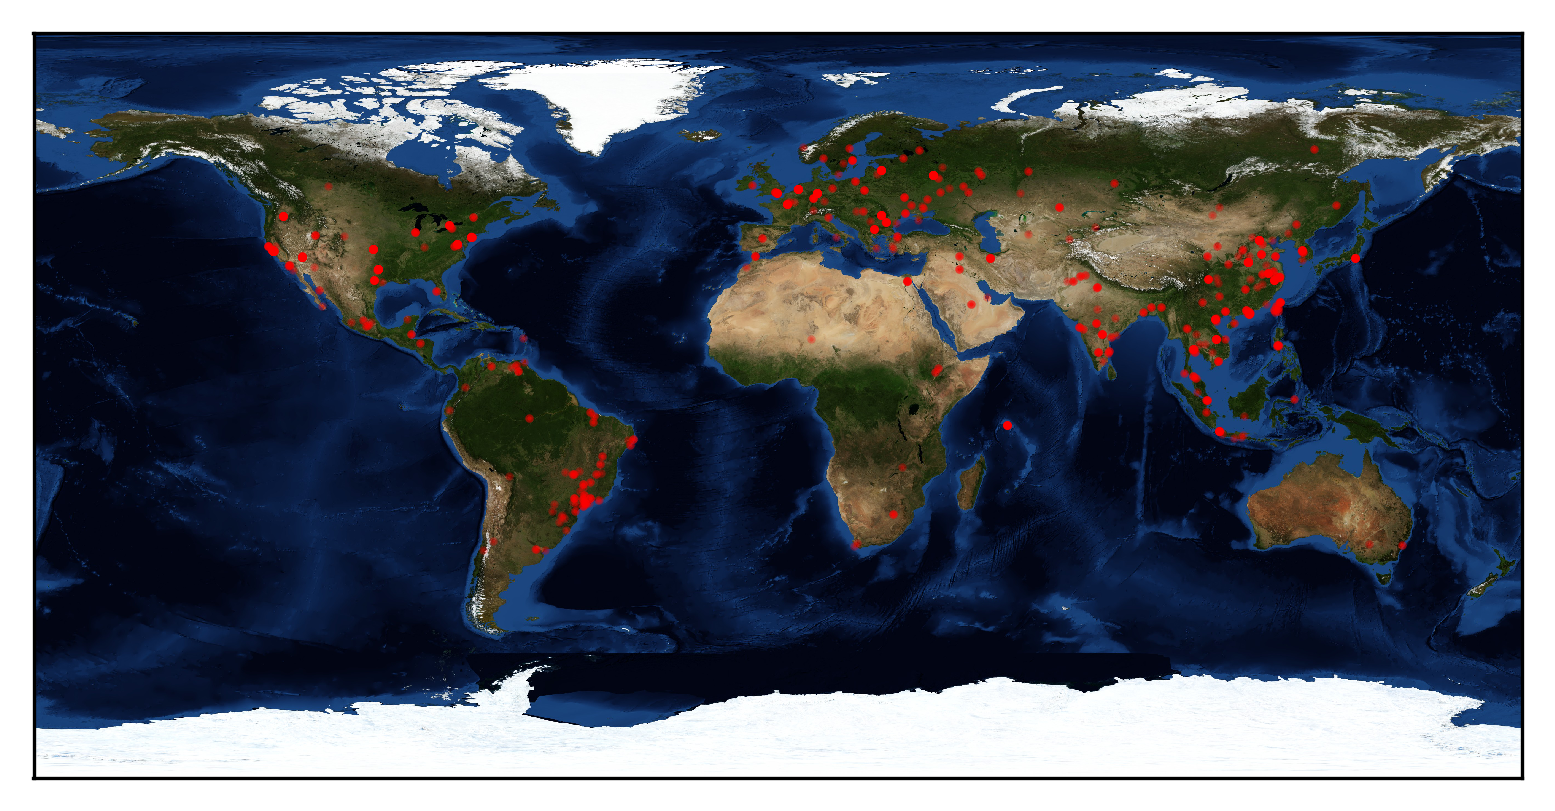
\includegraphics[width=\linewidth]{output.png}
	\caption{Approximate Locations of Attacker IP Addresses.}
	\label{fig:map}
\end{figure}


\section{Considerations}
\label{sec:considerations}
Since we are using AWS to host our honeypot, we must consider the configuration of the AWS instance itself. In particular, we will consider AWS firewall rules and security groups to allow all incoming connections and deny all outgoing connections. We must also consider that AWS might shutdown our server if they detect it is under attack. In that case, we will have a backup of the server prepared and it will be migrated to a private server which we control. Finally, if our honeypot does not collect enough attack data in the time period during which it is active, we will attack the server ourselves to demonstrate its capabilities. 

If time permits, we have further plans to add more AWS honeypot servers and network them together with our original instance to hopefully see how an attack might traverse the network. We can also implement an intrusion detection system such as \href{https://www.snort.org/}{Snort}if we have enough time. 

\section{Related Work}
\label{sec:related}

Point out other important approaches in the problem area. For example, if you 
are proposing an architecture, maybe OS or PL approaches to this problem. 

The following paragraph included just for a figure. The caption of a figure is very
important -- I try to tell the entire story in the figures and captions alone, 
just in case that is all the reader sees.

The general problem of determining whether information flows in a program from
variable $x$ to variable $y$ is undecidable, as ``any procedure purported to
decide it could be applied to the statement {\bf if}~$f(x)$~halts {\bf then}~$y
:= 0$ and thus provide a solution to the halting problem for arbitrary
recursive function''~\cite{denning-impossible}.  


\section{Conclusions}
\label{sec:conclusion}
In order to research the effectiveness of honeypots, we implemented and configured our own honeypot on an AWS server. Our honeypot collected even more data than we expected over the course of a single week. We have analyzed the data collected by our honeypot to find trends in the origin of attacks, the hardware used for attacks, which services are most heavily targeted, and more. Thus, our research has demonstrated that honeypots are an effective tool for monitoring malicious activity on a network. Our research also shows that honeypots can collect large amounts of data on many different types of trends. The data collected by a honeypot can be tailored to suit any organizations specific needs, making honeypots an effective tool not only for research, but also for securing enterprise environments. 

%\section{References}


{ 
\bibliographystyle{abbrv}
\bibliography{biblio}
}
%[1] Mairh, Abhishek \& Barik, Debabrat \& Verma, Kanchan \& Jena, Debasish. (2011). Honeypot in network security: A survey. ACM International Conference Proceeding Series. 600-605. 10.1145/1947940.1948065. \linebreak

%[2] Chuvakin, A. (2003). “Honeynets: High Value Security Data”: Analysis of real attacks launched at a honeypot. Network Security, 2003(8), 11-15. \linebreak

%[3] Gathof, S. (2018). Deploying a Honeypot on AWS [Blog post]. Retrieved from \href{https://medium.com/@sudojune/deploying-a-honeypot-on-aws-5bb414753f32}{https://medium.com/
%	\linebreak@sudojune/deploying-a-honeypot-on-aws-5bb414753f32}\linebreak

%[4] Polyakov, V. V., \& Lapin, S. A. (2018, October). Architecture of the Honeypot System for Studying Targeted Attacks. In 2018 XIV International Scientific-Technical Conference on Actual Problems of Electronics Instrument Engineering (APEIE) (pp. 202-205). IEEE.

%[5] N. Fox, “Setting up dionaea \& cowrie with mhn,” Malware, Threat Hunting \& Incident Response, 24-Sep-2019. [Online]. Available: https://neil-fox.github.io/Setting-up-Dionaea-\&-Cowrie-with-MHN/. [Accessed: 04-Dec-2019].

\end {document}

